%!TEX root = ../dissertation.tex

\section{Epipolar Geometry}
\label{cha2:epipolar}

Epipolar geometry provides an alternative yet powerful tool to obtain image transformations. It describes the relation between two views of a single scene through a 3x3 singular, non-invertible, matrix called the \textbf{essential matrix}, \textbf{$E$}, if the camera matrix is known, or the \textbf{fundamental matrix}, \textbf{$F$}, otherwise. These matrices are singular because they express an underconstrained relationship between a point in one image and its possible location in the other image, which is not unique due to depth ambiguity. The essential matrix is the product of a rotation matrix and a skew-symmetric matrix, whose determinant is zero, as it will be shown below. If a point in the (3D) world, $M$, is projected as point $\mathbf{{m}_1}$ in the first view, and point $\mathbf{{m}_2}$ in the second, then those points satisfy the relation

\begin{equation}
\label{sec2:eq:epipolar}
\mathbf{\tilde{m}_2}^T F \mathbf{\tilde{m}_1} = 0.
\end{equation}

\begin{figure}[h]
	\centering
	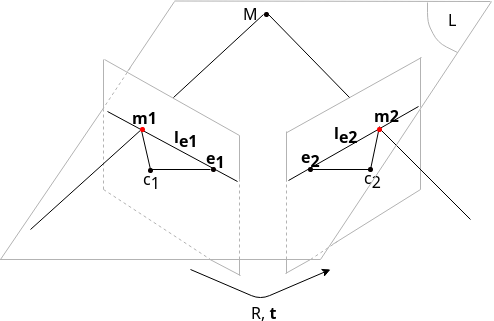
\includegraphics[width=10cm]{images/epipolargeo.png}
	\caption[Epipolar geometry]{Epipolar geometry. The two small planes correspond to the image planes of two different views by the camera, separated by a rotation $R$ and a translation $\bf t$, of the same scene, with centers of projection given by $c_1$ and $c_2$, respectively. $M$ is the fixed point gazed at in the real world. $\bf m_1$ and $\bf m_2$ are the projections of point $M$ into the respective image planes, whose rays are lying on the plane $L$. $\bf l_{e1}$ and $\bf l_{e2}$ are the epipolar lines, that also lie on the plane and $\bf e_1$ and $\bf e_2$ are the epipoles. The line defined by the centers is called the baseline.}
	\label{sec2:fig:epipolargeo}
\end{figure}


In Figure \ref{sec2:fig:epipolargeo}, $c_1$ and $c_2$ are the centers of projection of the first and second views of the scene from one camera that has been displaced by $(R, \mathbf{t})$ (or by two cameras staring at the same scene). Given the point on the first view, $\bf m_1$, its correspondence to the second view is constrained to a line, which is called the epipolar line, $\bf l_{e2}$. This line is defined as the intersection of the plane $L$ and the second view's image plane. Furthermore, plane $L$ is delineated by the centers of projection of both views and $\bf m_1$. The epipoles, $\bf e_1$ and $\bf e_2$, are born from the intersection of the line $c_1 - c_2$ (baseline) with the epipolar lines, $\bf l_{e1}$ and $\bf l_{e2}$. 

\subsection{Projective geometry concepts}

\subsubsection{Homogenous representation of lines}
A line in a plane is represented by $a x + b y + c = 0$, which can also be defined by a vector $( a , b , c ) ^T$. For any non-zero constant, $k$, the vectors  $( a , b , c ) ^T$ and $k(a , b , c ) ^T$ represent the same line and are equivalent. An equivalence class of vectors is known as an homogenous vector. 

\subsubsection{Point lying on a line}

A point $\mathbf { m } = ( x , y ) ^ T$ lies on a line $\mathbf {\tilde{l}} = ( a , b , c ) ^ { T }$, if and only if $a x + b y + c = 0$, which can be written as $( x , y , 1 ) ( a , b , c ) ^T = \mathbf { \tilde{m} } ^T \mathbf {\tilde{l}} = \mathbf {\tilde{l}} ^T \mathbf { \tilde{m} } = 0$.

\subsubsection{Line joining points}
A line passing through any two points $\mathbf{m}$ and $\mathbf{m'}$ can be defined by the cross-product of those points as $\mathbf{\tilde{l}} = \mathbf{\tilde{m}} \times \mathbf{\tilde{m}'}$.

\subsubsection{Cross product's skew symmetric representation}
The previous cross product, $\mathbf{\tilde{l}} = \mathbf{\tilde{m}} \times \mathbf{\tilde{m}'}$, can be written as $\mathbf{\tilde{l}} = [\mathbf{\tilde{m}}]_{\times} \mathbf{\tilde{m}'}$, where $[\mathbf{\tilde{m}}]_{\times}$ is defined as
\begin{equation}
\label{sec2:eq:crossp}
\left[ \mathbf{\tilde{m}} \right]_ { \times } =  \left[ \begin{array} { c c c } { 0 } & { - m _ { 3 } } & { m _ { 2 } } \\ { m _ { 3 } } & { 0 } & { - m _ { 1 } } \\ { - m _ { 2 } } & { m _ { 1 } } & { 0 } \end{array} \right].
\end{equation}

\subsection{Deducing the fundamental matrix}

With the above concepts, the following conclusions may be drawn:
\begin{enumerate}
	\item There is an homographic mapping via $L$ plane from the points of the first to the second view, characterized by $\mathbf{\tilde{m}_2} = H_M \mathbf{\tilde{m}_1}$;
	\item Because $\mathbf{m_2}$ lies on $\mathbf{\tilde{l}_2}$, then $\mathbf{ \tilde{m}_2 } ^T \mathbf{\tilde{l}_2} = 0$;
	\item Since $\mathbf { e_2 }, \mathbf { m_2 } \in \mathbf{\tilde{l}_2}$, then $\mathbf{\tilde{l}_2} = [\mathbf{\tilde{e}_2}]_{\times} \mathbf{\tilde{m}_2}$.
\end{enumerate}
From conclusions 1) and 3), 
\begin{equation}
\label{ggg}
\mathbf{\tilde{l}_2} = [\mathbf{\tilde{e}_2}]_{\times} H_M \mathbf{\tilde{m}_1} 
\end{equation}
can be deduced. Using conclusion 2) and (\ref{ggg}) 
\begin{equation}
\label{sec2:eq:fundm}
\mathbf{\tilde{m}_2}^T \mathbf{\tilde{l}_2} = 0 = \mathbf{\tilde{m}_2}^T [\mathbf{\tilde{e}_2}]_{\times} H_M \mathbf{\tilde{m}_1}  = \mathbf{\tilde{m}_2}^T F \mathbf{\tilde{m}_1} 
\end{equation}
$F$ is an homogeneous matrix of rank-2 (since $[\mathbf{\tilde{e}_2}]_{\times}$ is rank-2 and $H_M$ is rank-3) with 7 degrees of freedom, and $det(F) = 0$.

\subsection{Relationship between the fundamental matrix and camera motion}
Algebraically, having $M$ expressed in the first camera's reference frame, under the camera model studied above, (\ref{sec2:eq:eproj}) can be deduced.

\begin{equation}
\label{sec2:eq:eproj}
\lambda_1 \mathbf{\tilde{m}_2} = K _1 [ I \ \mathbf{0} ] \tilde{M}, \
\lambda_2 \mathbf{\tilde{m}_2} = K_2 [ R \ \mathbf{t} ] \tilde{M}
\end{equation}
In the case of only one camera in two different views: $K_1 = K_2$. For simplicity, the focal distance will be considered one meter, thus $K= I$ and the scale factors $\lambda_2$ and $\lambda_1$ will be dropped.
Now by eliminating $\tilde{M}$, the previous equation becomes
\begin{equation}
\label{sec2:eq:elimp}
\mathbf{\tilde{m}_2} = R   \mathbf{\tilde{m}_1} + \mathbf{t},
\end{equation}
and because the cross product of two vectors is orthogonal to them both,  
\begin{align}
	\label{sec2:eq:fundm1}
	\mathbf{\tilde{m}_2}^T \cdot ( \mathbf{\tilde{m}_2} \times \mathbf{t}) = 0 \\
	\label{sec2:eq:fundm2}
	( \mathbf{\tilde{m}_2}^T\cdot((R  \mathbf{\tilde{m}_1} + \mathbf{t}) \times \mathbf{t}) = 0,
\end{align}
the fundamental matrix, $F$, can be determined by 
\begin{equation}
\label{sec2:eq:fundm3}
\begin{aligned}
\mathbf{\tilde{m_2}}^T [\mathbf{t}]_\times R \mathbf{\tilde{m_1}} = 0 \\
\mathbf{\tilde{m_2}}^T F \mathbf{\tilde{m_1}} = 0.
\end{aligned}
\end{equation}
If the intrinsic parameters are not the identity matrix, then 
\begin{equation}
\begin{aligned}
\label{hhh}
\mathbf{\tilde{m_2}}^T K_2^{-T} E K_1^{-1} \mathbf{\tilde{m_1}} = 0 \\
F = K_2^{-T}  E K_1^{-1},
\end{aligned}
\end{equation}
where $E$ is the essential matrix.

\subsection{Estimating the fundamental matrix}
\label{einvonrev}
In order to find the fundamental matrix, and consequently the transformation from one view to another, having a set of matched image points, $\mathbf{m_{i1}} = [u_{1} \ v_{1}]^T$ and $\mathbf{m_{2}} = [u_{i2}  \ v_{2}]^T$, the epipolar equation (\ref{sec2:eq:epipolar}) can be written as
\begin{equation}
\begin{aligned}
\begin{bmatrix}
u_2 & v_2 & 1
\end{bmatrix}
\begin{bmatrix}
f_{11} & f_{12} & f_{13}  \\
f_{21} & f_{22} & f_{23}  \\
f_{31} & f_{32} & f_{33} 
\end{bmatrix}
\begin{bmatrix}
u_{1} \\ v_{1} \\ 1
\end{bmatrix}\\
=
\begin{bmatrix}
f_{11} u_1 u_2 + f_{12} v_1 u_2  + f_{13}u_2 + f_{21} u_1 v_2  + f_{22} v_1 v_2  + f_{23}v_2  + f_{31} u_1 + f_{32} v_1 + f_{33} 
\end{bmatrix}\\
=
\begin{bmatrix}
u_1u_2 \ v_1u_2 \ u_2 \ u_1v_2 \ v_1v_2 \  v_2 \ u_1 \ v_1 \ 1 
\end{bmatrix}
\begin{bmatrix}
f_{11} \ f_{12} \ f_{13} \ f_{21} \ f_{22} \ f_{23} \ f_{31} \ f_{32} \ f_{33}
\end{bmatrix}^T\\
= \mathbf{u} \cdot \mathbf{f}\\ = 0
\end{aligned}
\end{equation}
For $n$ sets of points the expression becomes 
\begin{equation}
\label{sec2:eq:nsets}
U f = 0,
\end{equation}
where $U = \left[ \mathbf{u_ { 1 }} , \cdots , \mathbf{u_ { n }} \right] ^ { T }$. 

This linear homogeneous equation, and the rank-2 constraint over $F$, that restrains the matrix to 7 degrees of freedom (since $F$ is also defined up a scalar factor), will permit its unique identification. 

The estimation of $F$ may be done using only 7 point matches, or by using 8 or more if enough data points are available. In the latter case, the solution produced is in general unique, and there are several techniques to obtain it. In Zhang 1996's review on the issue \cite{detep}, the conclusion was that linear techniques are usually sensitive to noise and not very stable, because they ignore the constraints of $F$ and the minimization criterion is not physically meaningful. However, the results could be improved by using normalized data points instead of pixel coordinates. 

Nevertheless, non-linear optimization techniques seem to yield better results to the estimation problem of $F$. Three nonlinear algorithms are available: (i) the distances between points and their corresponding epipolar lines, (ii) the gradient-weighted epipolar errors, and (iii) the distances between points and the reprojections of their corresponding points reconstructed in space. The third one is the most time-consuming method, thus not recommended. The first seems to give the worst results out of the three. Therefore, the second algorithm has been proposed to give the best results in the least amount of computational time.

Note that outliers, such as a wrongly matched pairs of points between the two views of the scene, or points with large location errors, could severely affect the precision of the estimation of $F$. The reason for this is that all methods are least-square techniques that assume the noise which corrupts the data has zero mean. Hence, more robust techniques have been proposed that are less sensitive to outliers, the most popular being M-estimators, and the least-median-of-squares (LMedS). The LMedS method solves a nonlinear minimization problem yielding the smallest value for
the median of squared residuals computed over the entire data set, and proves to be very robust both against false matches, and to erroneous locations, whereas M-estimators is less robust to false matches. LMedS must be solved by a search in the space of possible estimates generated from the data, which is too time-consuming. Thus, as a pragmatic approach is to only test a random sample of the data.\\

\subsection{Factorization of the essential matrix}

Once the fundamental matrix is obtained through one of those methods, assuming the intrinsic parameters are known, which is the case for this project, where the setup is only one camera, the essential matrix may be obtained by $E = K^{T}  F K$ as seen on (\ref{hhh}).
From here, it's possible to retrieve the camera matrix, $P = [R \ | \ \mathbf{t}]$ from the first to the second view, since $E = [\mathbf{t}]_\times R$. 

A $3x3$ matrix is an essential matrix if and only if two of its singular values are equal, and the third is zero. This is easily proven by the decomposition of $E = SR$, where $S$ is a skew-symmetric matrix, as follows.
Considering matrices 
\begin{equation}
\mathrm { W } = \left[ \begin{array} { c c c } { 0 } & { - 1 } & { 0 } \\ { 1 } & { 0 } & { 0 } \\ { 0 } & { 0 } & { 1 } \end{array} \right] \quad \text { and } \quad \mathrm { Z } = \left[ \begin{array} { c c c } { 0 } & { 1 } & { 0 } \\ { - 1 } & { 0 } & { 0 } \\ { 0 } & { 0 } & { 0 } \end{array} \right],
\end{equation}
where $W$ is orthogonal and $Z$ is skew-symmetric, $S$ may be written as\footnote{A proof of this is given in Result A4.1 of R. Hartley and A. Zisserman,Multiple View Geometry in Computer Vision \cite{epipolar}} $S = kUZU^T$, where $U$ is orthogonal and $Z = \operatorname{diag}(1,1,0)W$, up to sign. Thus, $S = U \operatorname { diag } ( 1,1,0 ) WU^T$, up to scale, and 
\begin{equation}
E = SR = U \operatorname { diag } ( 1,1,0 ) \left( WU^T R \right) = U \operatorname { diag } ( 1,1,0 ) V^T,
\end{equation}
proving the initial statement.

Because the singular values have to be equal, the SVD of $E$ is not unique, in fact 
\begin{equation}
\label{gf}
E = U \operatorname { diag } ( 1,1,0 ) V ^ { T },
\end{equation}
or 
\begin{equation}
E = U \operatorname { diag } ( 1,1,0 ) ( - V ) ^ { T }.
\end{equation} 
Considering (\ref{gf}), because
\begin{equation}
\begin{aligned} 
Z W = \operatorname { diag } ( 1,1,0 ) \\ 
\text{and} \
Z W ^ { T } = - \operatorname { diag } ( 1,1,0 ) ,
\end{aligned}
\end{equation}
$E=SR$ may be decomposed into two forms,
\begin{equation}
\label{ccha}
S = - U Z U ^ { T } , \quad R = U W ^ { T } V ^ { T },
\end{equation}
or
\begin{equation}
\label{ccha2}
S = U Z U ^ { T } , \quad R = U W V ^ { T }.
\end{equation}
The matrix $R$ on (\ref{ccha}) is a rotation, since it is orthogonal,
\begin{equation}
R ^ { T } R = \left( U W ^ { T } V ^ { T } \right) ^ { T } U W ^ { T } V ^ { T } = V W U ^ { T } U W ^ { T } V ^ { T } = I,
\end{equation}
and 
\begin{equation}
\operatorname { det } \left( U W ^ { T } V ^ { T } \right) = \operatorname { det } ( U ) \operatorname { det } \left( W ^ { T } \right) \operatorname { det } \left( V ^ { T } \right) = \operatorname { det } ( W ) \operatorname { det } \left( U V ^ { T } \right) = 1,
\end{equation}
which are enough conditions to prove it. Furthermore, $S$ is skew-symmetric because,
\begin{equation}
- S^ { T } = \left( U Z U ^ { T } \right) ^ { T } = U Z ^ { T } U ^ { T } = - U Z U ^ { T } = S.
\end{equation}
The same applies to (\ref{ccha2}). \cite{lecture} A proof that these are the only solutions is given in Result 9.18 of R. Hartley and A. Zisserman \cite{epipolar}.

Now regarding the translation, since $S \mathbf{t} = [\mathbf{t}]_{\times}\mathbf{t} = 0$, it follows that $t = U (0, 0, 1)^T = u_3$, the last column of $U$, which can be explained by the following. Assuming $S \mathbf{t} = U Z U^T \mathbf{t} = 0$, $Z U^T \mathbf{t}$ should be equal to zero to satisfy the equation. Because $Z$ is an orthogonal matrix,
\begin{equation}
Z U^T \mathbf{t} = \left[ \begin{array} { c c c } { 0 } & { 1 } & { 0 } \\ { - 1 } & { 0 } & { 0 } \\ { 0 } & { 0 } & { 0 } \end{array} \right] U^T \mathbf{t}  = \left[ \begin{array} { c c c } { 0 } & { 1 } & { 0 } \\ { - 1 } & { 0 } & { 0 } \\ { 0 } & { 0 } & { 0 } \end{array} \right] \left[ \begin{array} { c } { 0 } \\ { 0} \\ s \end{array} \right] = 0,
\end{equation}
where $s$ is any non-zero constant, such as $1$. Therefore, $\mathbf{t} = U [0 \ 0 \ 1]^T = u_3$, as U is orthogonal as well.\\
Finally, due to the lack of uniqueness of the SVD, there are 4 possible solutions for the camera matrix,
\begin{equation}
P = \left[UWV^T | + u_{ 3 } \right] \quad \text { or } \quad \left[ UWV^T | - u_ { 3 } \right] \quad \text { or } \quad \left[ UW^T V^T | + u_ { 3 } \right] \quad \text { or } \quad \left[ UW^T V^T |- u _ { 3 } \right],
\end{equation}
that are represented by (a), (b), (c) and (d), respectively, on Figure \ref{sec2:fig:ep4}. 

\begin{figure}[ht]
	\centering
	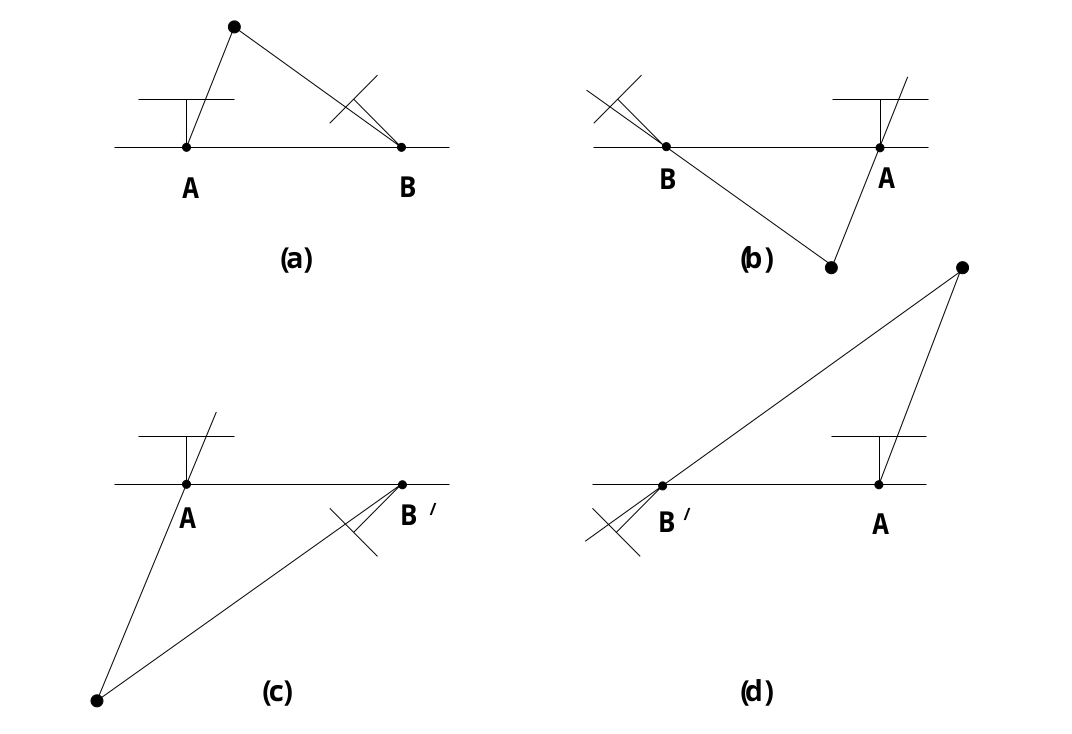
\includegraphics[width=10cm]{images/ep4sols.png}
	\caption[Four possible solutions retrieved from $E$]{Four possible solutions retrieved from $E$. A and B are the first and second camera center positions when looking at the same scene. Between the right side, (a) and (c), and the left side, (b) and (d), figures, there is a translation direction inversion. Between top, (a) and (b), and bottom, (c) and (d), figures, there is a rotation of 180 degrees around the baseline. \cite{epipolar}}
	\label{sec2:fig:ep4}
\end{figure}
The real world point is only in front of both cameras in one of the four solutions, thus, it is enough to use a single point to decide which of the different solutions produces the correct camera matrix. \cite{epipolar}

To summarize, the steps for obtaining the projective transformation from epipolar geometry are:
\begin{enumerate}
	\item Determining the fundamental matrix, $F$, using one of the algorithms described on section \ref{einvonrev};
	\item Obtain the essential matrix, $E$, from the intrinsic parameters (which is possible in this case);
	\item Retrieve the four possible solutions for $P = [R \ \mathbf{t}]$ by doing a SVD decomposition on $E$;
	\item Choose the feasible solution.
\end{enumerate}